\section{Controller Tuning and Model Parameter Estimation}\label{sec:prob1}
\label{text:problem1}

\subsection{PID-tuning}
The pre-tuned PID controllers showed unsatisfactory performance and was re-tuned to better serve as the stable plant for the rest of the assignment. In particular, the pre-tuned pitch controller was tuned in an aggressive fashion, impacting elevation control significantly. Figure \ref{fig:pid_tuning} shows the coupling of pitch and elevation control before and after tuning. The two controllers were tuned independently of each other, in a manual fashion.

\begin{table}[hp]
	\centering
	\caption{Controller gains comparison}
	\begin{tabular}{llll}
		\hline
		Gain & Original & Improved \\
		\hline
		$K_{pp}$ & 93.2 & 14.0 \\
		$K_{pd}$ & 13.2 & 2.5 \\
		$K_{ei}$ & 2.3 & 2.3 \\
		$K_{ep}$ & 7.0 & 15.0 \\
		$K_{ed}$ & 10.0 & 13.0 \\
	\end{tabular}
	\label{tab:gains}
\end{table}

\begin{figure}[hp]
	\centering
		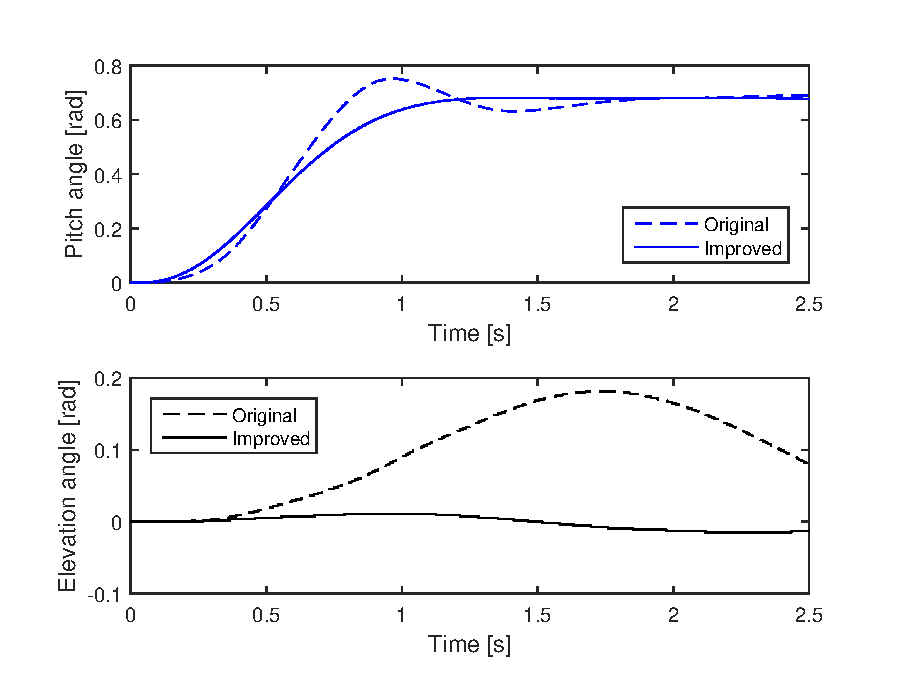
\includegraphics[width=0.85\textwidth]{figures/1/pid_tuning.eps}
	\caption{Pitch and elevation response to pitch step input, with original and improved pitch and elevation controller tuning.}
	\label{fig:pid_tuning}
\end{figure}


\subsection{Model parameter estimation}
The derived model in \eqref{eq:dynamics} showed considerably different dynamics than the observed ones. The system identification toolbox in MATLAB was therefore used to compute the parameters which fitted the recorded step responses. This was done by estimating the following three step responses based on known input and recorded system behavior:

\begin{itemize}
	\item{Pitch setpoint to pitch}
	\item{Elevation setpoint to elevation}
	\item{Pitch to travel rate}
\end{itemize}

Figure \ref{fig:pitch_model_comparison} shows the pitch step response of the derived model compared with the newly estimated model, and the measured step response. The estimated model is clearly a better match than the derived model. Optimal input sequences calculated based on the derived model would need extensive help from feedback in order to yield usable performance. The elevation step responses of the derived and estimated model, shown in figure \ref{fig:elev_model_comparison}, and travel rate response in figure \ref{fig:travelRate_model_comparison}, displays similar results.

\begin{figure}[hp]
	\centering
		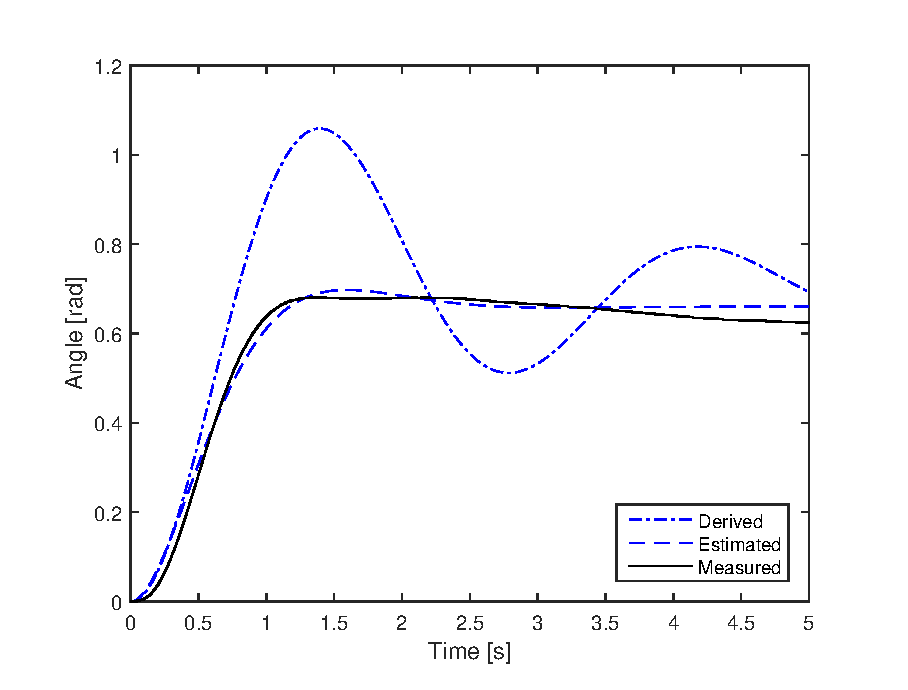
\includegraphics[width=0.85\textwidth]{figures/1/pitch_model_comparison.eps}
	\caption{Pitch step responses of the derived and estimated model, compared with the measured step response.}
	\label{fig:pitch_model_comparison}
\end{figure}

\begin{figure}[hp]
	\centering
		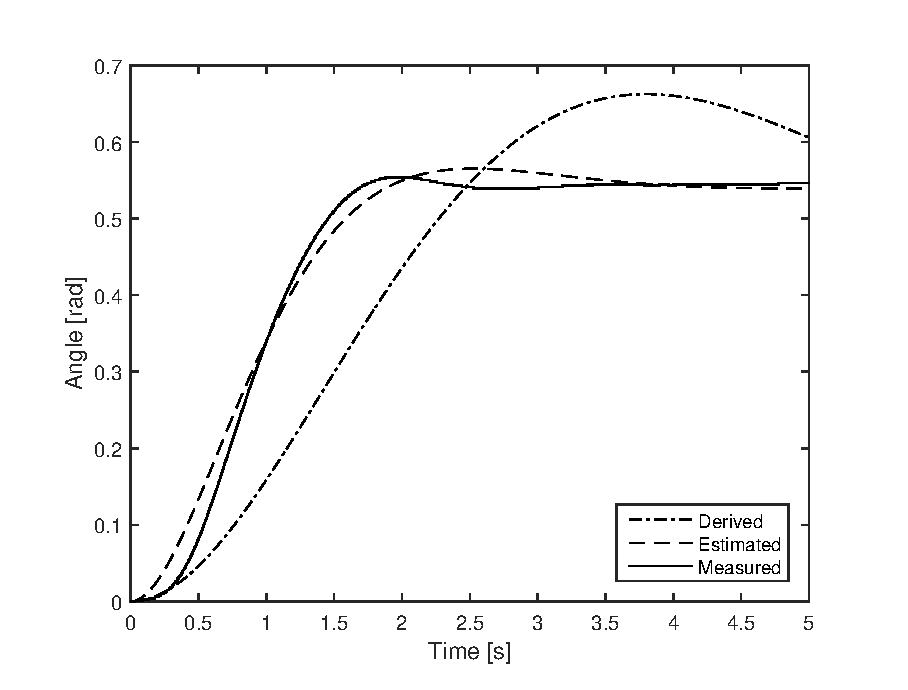
\includegraphics[width=0.85\textwidth]{figures/1/elev_model_comparison.eps}
	\caption{Elevation step responses of the derived and estimated model, compared with the measured step response.}
	\label{fig:elev_model_comparison}
\end{figure}

\begin{figure}[hp]
	\centering
		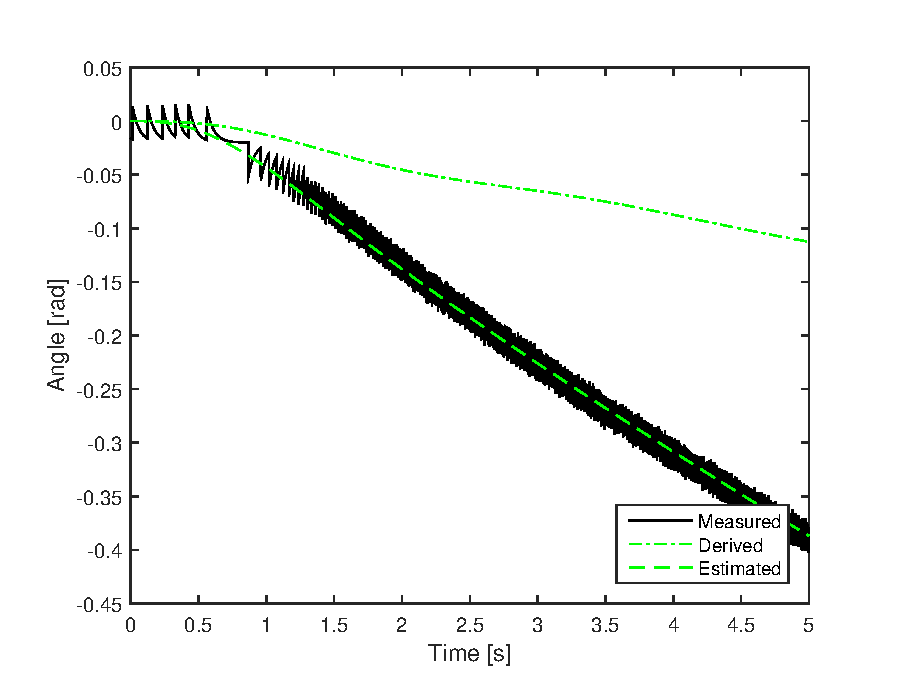
\includegraphics[width=0.85\textwidth]{figures/1/travelRate_model_comparison.eps}
	\caption{Travel rate response of commanded step in pitch. Derived and estimated model compared with the measured response.}
	\label{fig:travelRate_model_comparison}
\end{figure}


\subsection{Results and discussion}
\label{subsection:part1_results}


The following transfer functions were estimated from measured step responses:

\begin{subequations}
\label{eq:tf}
\begin{align}
	\frac{p}{p_c}(s) &= \frac{6.74}{s^2 + 3.60 s + 7.13},\label{eq:p_pc}\\
	\frac{e}{e_c}(s) &= \frac{3.13}{s^2 + 2.45 s + 3.03},\label{eq:e_ec}\\
	\frac{\lambda}{p}(s) &= \frac{-0.29}{s + 0.05}.\label{eq:travelRate_p}
\end{align}
\end{subequations}


The calculated response of the travel rate in figure \ref{fig:travelRate_model_comparison} is almost identical to the recorded step response. The pitch and elevation models are satisfactory, but the dynamics are clearly not matching the actual dynamics to the same degree as with travel rate. This should be expected, as the small angle approximation used is bound to yield errors, especially in the pitch model. Both the off-axis hinged pitch head and the non-linearity of rotor thrust are also unaccounted for when settling on the number of states. A third state for both pitch and elevation might have helped capture some of the dynamics, but as we want to minimize the number of states, the results are found to be well within acceptable levels.



